\documentclass[11pt]{article}\usepackage[]{graphicx}\usepackage[]{color}
%% maxwidth is the original width if it is less than linewidth
%% otherwise use linewidth (to make sure the graphics do not exceed the margin)
\makeatletter
\def\maxwidth{ %
  \ifdim\Gin@nat@width>\linewidth
    \linewidth
  \else
    \Gin@nat@width
  \fi
}
\makeatother

\definecolor{fgcolor}{rgb}{0.345, 0.345, 0.345}
\newcommand{\hlnum}[1]{\textcolor[rgb]{0.686,0.059,0.569}{#1}}%
\newcommand{\hlstr}[1]{\textcolor[rgb]{0.192,0.494,0.8}{#1}}%
\newcommand{\hlcom}[1]{\textcolor[rgb]{0.678,0.584,0.686}{\textit{#1}}}%
\newcommand{\hlopt}[1]{\textcolor[rgb]{0,0,0}{#1}}%
\newcommand{\hlstd}[1]{\textcolor[rgb]{0.345,0.345,0.345}{#1}}%
\newcommand{\hlkwa}[1]{\textcolor[rgb]{0.161,0.373,0.58}{\textbf{#1}}}%
\newcommand{\hlkwb}[1]{\textcolor[rgb]{0.69,0.353,0.396}{#1}}%
\newcommand{\hlkwc}[1]{\textcolor[rgb]{0.333,0.667,0.333}{#1}}%
\newcommand{\hlkwd}[1]{\textcolor[rgb]{0.737,0.353,0.396}{\textbf{#1}}}%

\usepackage{framed}
\makeatletter
\newenvironment{kframe}{%
 \def\at@end@of@kframe{}%
 \ifinner\ifhmode%
  \def\at@end@of@kframe{\end{minipage}}%
  \begin{minipage}{\columnwidth}%
 \fi\fi%
 \def\FrameCommand##1{\hskip\@totalleftmargin \hskip-\fboxsep
 \colorbox{shadecolor}{##1}\hskip-\fboxsep
     % There is no \\@totalrightmargin, so:
     \hskip-\linewidth \hskip-\@totalleftmargin \hskip\columnwidth}%
 \MakeFramed {\advance\hsize-\width
   \@totalleftmargin\z@ \linewidth\hsize
   \@setminipage}}%
 {\par\unskip\endMakeFramed%
 \at@end@of@kframe}
\makeatother

\definecolor{shadecolor}{rgb}{.97, .97, .97}
\definecolor{messagecolor}{rgb}{0, 0, 0}
\definecolor{warningcolor}{rgb}{1, 0, 1}
\definecolor{errorcolor}{rgb}{1, 0, 0}
\newenvironment{knitrout}{}{} % an empty environment to be redefined in TeX

\usepackage{alltt}
\usepackage{amsmath}
\usepackage{listings}
\usepackage{stmaryrd}
\usepackage{bbm}
\usepackage{amsmath}
\usepackage{mathtools}
\usepackage{pdfpages}
\usepackage{breqn}



\newcount\colveccount
\newcommand*\colvec[1]{
        \global\colveccount#1
        \begin{pmatrix}
        \colvecnext
}
\def\colvecnext#1{
        #1
        \global\advance\colveccount-1
        \ifnum\colveccount>0
                \\
                \expandafter\colvecnext
        \else
                \end{pmatrix}
        \fi
}
\newcommand{\argmin}{\arg\!\min}

\author{Thibault Doutre, Student ID 26980469}
\title{STAT230 HW 10 \\
University of California, Berkeley}
\date{\today}
\IfFileExists{upquote.sty}{\usepackage{upquote}}{}
\begin{document}

\maketitle
\section{}
\begin{knitrout}
\definecolor{shadecolor}{rgb}{0.969, 0.969, 0.969}\color{fgcolor}\begin{kframe}
\begin{alltt}
\hlcom{# Load data ----------------------------------------------}

\hlkwd{load}\hlstd{(}\hlstr{"HW10.rda"}\hlstd{)}

\hlcom{## shuffle}
\hlstd{data} \hlkwb{=} \hlstd{data[}\hlkwd{sample}\hlstd{(}\hlkwd{nrow}\hlstd{(data)),]}

\hlcom{# Full Model, R2 -----------------------------------------}

\hlcom{## # OLS fit}
\hlstd{lm.fit} \hlkwb{=} \hlkwd{lm}\hlstd{(Y}\hlopt{~}\hlstd{.,} \hlkwc{data}\hlstd{=data)}

\hlcom{## # R2}
\hlstd{R2} \hlkwb{=} \hlkwd{var}\hlstd{(lm.fit}\hlopt{$}\hlstd{fitted.values)}\hlopt{/}\hlkwd{var}\hlstd{(data}\hlopt{$}\hlstd{Y)}
\hlstd{R2}
\end{alltt}
\begin{lstlisting}[basicstyle=\ttfamily,breaklines=true]
## [1] 0.5011678
\end{lstlisting}
\begin{alltt}
\hlcom{## # Cross validated R2}

\hlstd{R2_cv} \hlkwb{=} \hlkwa{function}\hlstd{(}\hlkwc{data}\hlstd{,} \hlkwc{nfold}\hlstd{,} \hlkwc{formula}\hlstd{=}\hlstr{"Y~."}\hlstd{)\{}
  \hlcom{# Compute R2 based on cross validated data}
  \hlstd{Y_cv} \hlkwb{=} \hlkwd{c}\hlstd{()}
  \hlstd{nrows} \hlkwb{=} \hlkwd{nrow}\hlstd{(data)}
  \hlkwa{for} \hlstd{(i} \hlkwa{in} \hlkwd{seq}\hlstd{(}\hlnum{0}\hlstd{, nrows}\hlopt{-}\hlstd{nfold,} \hlkwc{by}\hlstd{=nrows}\hlopt{/}\hlstd{nfold))\{}
    \hlkwd{print}\hlstd{(i}\hlopt{+}\hlnum{1}\hlstd{)}
    \hlkwd{print}\hlstd{(nfold}\hlopt{+}\hlstd{i)}
    \hlstd{test} \hlkwb{=} \hlstd{i}\hlopt{:}\hlstd{(nfold}\hlopt{+}\hlstd{i)}
    \hlstd{train} \hlkwb{=} \hlopt{-}\hlstd{test}
    \hlstd{lm.fit} \hlkwb{=} \hlkwd{lm}\hlstd{(formula,} \hlkwc{data}\hlstd{=data[train,])}
    \hlstd{Ytest} \hlkwb{=} \hlkwd{predict}\hlstd{(lm.fit, data[test,])}
    \hlstd{Y_cv} \hlkwb{=} \hlkwd{c}\hlstd{(Y_cv, Ytest)}
  \hlstd{\}}
  \hlkwd{var}\hlstd{(Y_cv)}\hlopt{/}\hlkwd{var}\hlstd{(data}\hlopt{$}\hlstd{Y)}
\hlstd{\}}
\hlkwd{names}\hlstd{(lm.fit)}
\end{alltt}
\begin{lstlisting}[basicstyle=\ttfamily,breaklines=true]
##  [1] "coefficients"  "residuals"     "effects"      
##  [4] "rank"          "fitted.values" "assign"       
##  [7] "qr"            "df.residual"   "xlevels"      
## [10] "call"          "terms"         "model"
\end{lstlisting}
\begin{alltt}
\hlstd{nfold} \hlkwb{=} \hlnum{10}
\hlstd{R2_cv10} \hlkwb{=} \hlkwd{R2_cv}\hlstd{(data,} \hlnum{10}\hlstd{)}
\end{alltt}
\begin{lstlisting}[basicstyle=\ttfamily,breaklines=true]
## [1] 1
## [1] 10
## [1] 11
## [1] 20
## [1] 21
## [1] 30
## [1] 31
## [1] 40
## [1] 41
## [1] 50
## [1] 51
## [1] 60
## [1] 61
## [1] 70
## [1] 71
## [1] 80
## [1] 81
## [1] 90
## [1] 91
## [1] 100
\end{lstlisting}
\begin{alltt}
\hlstd{R2_cv10}
\end{alltt}
\begin{lstlisting}[basicstyle=\ttfamily,breaklines=true]
## [1] 0.591366
\end{lstlisting}
\begin{alltt}
\hlkwd{summary}\hlstd{(lm.fit)}
\end{alltt}
\begin{lstlisting}[basicstyle=\ttfamily,breaklines=true]
## 
## Call:
## lm(formula = Y ~ ., data = data)
## 
## Residuals:
##     Min      1Q  Median      3Q     Max 
## -2.2462 -0.7195  0.0226  0.5911  3.3454 
## 
## Coefficients:
##             Estimate Std. Error t value Pr(>|t|)    
## (Intercept)  0.44742    0.12700   3.523 0.000713 ***
## f            0.31565    0.12122   2.604 0.011008 *  
## d            0.45784    0.13563   3.376 0.001145 ** 
## t            0.22951    0.11538   1.989 0.050135 .  
## a            0.36626    0.14114   2.595 0.011272 *  
## i            0.07495    0.14521   0.516 0.607209    
## n            0.09645    0.12999   0.742 0.460307    
## l            0.21065    0.12259   1.718 0.089666 .  
## q            0.07316    0.12947   0.565 0.573640    
## e            0.49904    0.13516   3.692 0.000407 ***
## h            0.33018    0.14225   2.321 0.022860 *  
## b            0.34986    0.12641   2.768 0.007030 ** 
## g            0.22757    0.11859   1.919 0.058596 .  
## c            0.30609    0.13616   2.248 0.027362 *  
## p            0.05387    0.12778   0.422 0.674470    
## r            0.19486    0.15407   1.265 0.209677    
## o            0.01688    0.11065   0.153 0.879164    
## m            0.06620    0.13204   0.501 0.617531    
## s            0.11640    0.14126   0.824 0.412407    
## j            0.09100    0.11559   0.787 0.433484    
## k            0.27364    0.12343   2.217 0.029504 *  
## ---
## Signif. codes:  
## 0 '***' 0.001 '**' 0.01 '*' 0.05 '.' 0.1 ' ' 1
## 
## Residual standard error: 1.109 on 79 degrees of freedom
## Multiple R-squared:  0.5012,	Adjusted R-squared:  0.3749 
## F-statistic: 3.968 on 20 and 79 DF,  p-value: 5.525e-06
\end{lstlisting}
\end{kframe}
\end{knitrout}
The cross validated $R^2$ is significantly higher than both the multiple and adjusted $R^2$. The $R^2$ computed with the fitted values is approximately equal to the multiple $R^2$ (precision $10^{-4}$).

\section{}

\begin{knitrout}
\definecolor{shadecolor}{rgb}{0.969, 0.969, 0.969}\color{fgcolor}\begin{kframe}
\begin{alltt}
\hlcom{# Backward selection --------------------------------------}

\hlcom{## # Cross validated MSE}

\hlstd{MSE_cv} \hlkwb{=} \hlkwa{function}\hlstd{(}\hlkwc{data}\hlstd{,} \hlkwc{nfold}\hlstd{,} \hlkwc{formula}\hlstd{=}\hlstr{"Y~."}\hlstd{)\{}
  \hlcom{# Compute R2 based on cross validated data}
  \hlstd{Y_cv} \hlkwb{=} \hlkwd{c}\hlstd{()}
  \hlstd{nrows} \hlkwb{=} \hlkwd{nrow}\hlstd{(data)}
  \hlstd{MSE_test} \hlkwb{=} \hlkwd{c}\hlstd{()}
  \hlstd{MSE_train} \hlkwb{=} \hlkwd{c}\hlstd{()}
  \hlkwa{for} \hlstd{(i} \hlkwa{in} \hlkwd{seq}\hlstd{(}\hlnum{0}\hlstd{, nrows}\hlopt{-}\hlstd{nfold,} \hlkwc{by}\hlstd{=nrows}\hlopt{/}\hlstd{nfold))\{}
    \hlstd{test} \hlkwb{=} \hlstd{(i}\hlopt{+}\hlnum{1}\hlstd{)}\hlopt{:}\hlstd{(nfold}\hlopt{+}\hlstd{i)}
    \hlstd{train} \hlkwb{=} \hlopt{-}\hlstd{test}
    \hlstd{lm.fit} \hlkwb{=} \hlkwd{lm}\hlstd{(formula,} \hlkwc{data}\hlstd{=data[train,])}
    \hlstd{Ytest} \hlkwb{=} \hlkwd{predict}\hlstd{(lm.fit, data[test,])}
    \hlstd{MSE_test} \hlkwb{=} \hlkwd{c}\hlstd{(MSE_test,} \hlkwd{mean}\hlstd{((data}\hlopt{$}\hlstd{Y[test]}\hlopt{-}\hlstd{Ytest)}\hlopt{^}\hlnum{2}\hlstd{))}
    \hlstd{MSE_train} \hlkwb{=} \hlkwd{c}\hlstd{(MSE_train,}
                  \hlkwd{mean}\hlstd{((data}\hlopt{$}\hlstd{Y[train]}\hlopt{-}\hlstd{lm.fit}\hlopt{$}\hlstd{fitted.values)}\hlopt{^}\hlnum{2}\hlstd{))}
  \hlstd{\}}
  \hlcom{# Training error based on best model}
  \hlcom{# Test error based on cross validation (mean)}
  \hlkwd{return}\hlstd{(}\hlkwd{list}\hlstd{(}\hlkwc{test} \hlstd{=} \hlkwd{mean}\hlstd{(MSE_test),} \hlkwc{train} \hlstd{=} \hlkwd{min}\hlstd{(MSE_train)))}

\hlstd{\}}

\hlkwd{MSE_cv}\hlstd{(data, nfold)}
\end{alltt}
\begin{lstlisting}[basicstyle=\ttfamily,breaklines=true]
## $test
## [1] 1.621213
## 
## $train
## [1] 0.8486754
\end{lstlisting}
\begin{alltt}
\hlcom{## # Remove less significant feature from lm.fit}

\hlstd{backward_lm} \hlkwb{=} \hlkwa{function}\hlstd{(}\hlkwc{data}\hlstd{)\{}
  \hlcom{# Initialize with OLS}
  \hlstd{formula} \hlkwb{=} \hlstr{"Y~."}
  \hlstd{lm.fit} \hlkwb{=} \hlkwd{lm}\hlstd{(formula,} \hlkwc{data}\hlstd{=data)}
  \hlcom{# Initialize outputs}
  \hlstd{MSE_train} \hlkwb{=} \hlkwd{c}\hlstd{()}
  \hlstd{MSE_test} \hlkwb{=} \hlkwd{c}\hlstd{()}
  \hlstd{next_to_remove} \hlkwb{=} \hlstr{""}
  \hlstd{variables} \hlkwb{=} \hlkwd{c}\hlstd{()}
  \hlkwa{while}\hlstd{(}\hlkwd{length}\hlstd{(}\hlkwd{names}\hlstd{(lm.fit}\hlopt{$}\hlstd{model))}\hlopt{>}\hlnum{1}\hlstd{)\{}
    \hlstd{MSE} \hlkwb{=} \hlkwd{MSE_cv}\hlstd{(data,} \hlnum{10}\hlstd{, formula)}
    \hlstd{MSE_train} \hlkwb{=} \hlkwd{c}\hlstd{(MSE_train, MSE}\hlopt{$}\hlstd{train)}
    \hlstd{MSE_test} \hlkwb{=} \hlkwd{c}\hlstd{(MSE_test, MSE}\hlopt{$}\hlstd{test)}
    \hlstd{t_values} \hlkwb{=} \hlkwd{coef}\hlstd{(}\hlkwd{summary}\hlstd{(lm.fit))[,} \hlstr{"t value"}\hlstd{]}
    \hlcom{# Variable with smallest t-value}
    \hlstd{next_to_remove} \hlkwb{=} \hlkwd{names}\hlstd{(}\hlkwd{which.min}\hlstd{(t_values))}
    \hlcom{# Store removed variables in the order}
    \hlstd{variables} \hlkwb{=} \hlkwd{c}\hlstd{(variables,next_to_remove)}
    \hlcom{# Update formula}
    \hlstd{formula} \hlkwb{=} \hlkwd{paste}\hlstd{(formula,}\hlstr{"-"}\hlstd{,next_to_remove,}\hlkwc{sep}\hlstd{=}\hlstr{""}\hlstd{)}
    \hlcom{# Update model using new formula}
    \hlstd{lm.fit} \hlkwb{=} \hlkwd{update}\hlstd{(lm.fit, formula)}
  \hlstd{\}}
  \hlcom{# Intercept only}
  \hlstd{MSE} \hlkwb{=} \hlkwd{MSE_cv}\hlstd{(data,} \hlnum{10}\hlstd{, formula)}
  \hlstd{MSE_train} \hlkwb{=} \hlkwd{c}\hlstd{(MSE_train, MSE}\hlopt{$}\hlstd{train)}
  \hlstd{MSE_test} \hlkwb{=} \hlkwd{c}\hlstd{(MSE_test, MSE}\hlopt{$}\hlstd{test)}
  \hlkwd{return}\hlstd{(}\hlkwd{list}\hlstd{(}\hlkwc{variables} \hlstd{= variables,} \hlkwc{MSE_test} \hlstd{= MSE_test,}
              \hlkwc{MSE_train} \hlstd{= MSE_train))}
\hlstd{\}}

\hlstd{backward} \hlkwb{=} \hlkwd{backward_lm}\hlstd{(data)}
\hlstd{backward}
\end{alltt}
\begin{lstlisting}[basicstyle=\ttfamily,breaklines=true]
## $variables
##  [1] "o" "p" "m" "q" "n" "j" "i" "s" "r" "l" "k" "t" "f" "b"
## [15] "a" "c" "g" "e" "h" "d"
## 
## $MSE_test
##  [1] 1.621213 1.570532 1.566042 1.497060 1.454698 1.424109
##  [7] 1.407780 1.391831 1.377380 1.366292 1.381277 1.409561
## [13] 1.450584 1.497906 1.534049 1.547914 1.643368 1.698750
## [19] 1.757956 1.851872 1.989268
## 
## $MSE_train
##  [1] 0.8486754 0.8515116 0.8515768 0.8557102 0.8611087
##  [6] 0.8766084 0.8815017 0.8881369 0.9108102 0.9304373
## [11] 0.9673466 0.9969965 1.0311388 1.0533816 1.0777200
## [16] 1.1727420 1.2694991 1.4019090 1.4794819 1.6056939
## [21] 1.7747474
\end{lstlisting}
\end{kframe}
\end{knitrout}


\section{}
\begin{knitrout}
\definecolor{shadecolor}{rgb}{0.969, 0.969, 0.969}\color{fgcolor}\begin{kframe}
\begin{alltt}
\hlcom{# Forward selection ----------------------------------------}

\hlstd{forward_lm} \hlkwb{=} \hlkwa{function}\hlstd{(}\hlkwc{data}\hlstd{)\{}
  \hlstd{names} \hlkwb{=} \hlkwd{names}\hlstd{(data)[}\hlopt{-}\hlnum{1}\hlstd{]}
  \hlcom{# Initialize outputs}
  \hlstd{MSE_train} \hlkwb{=} \hlkwd{c}\hlstd{()}
  \hlstd{MSE_test} \hlkwb{=} \hlkwd{c}\hlstd{()}
  \hlstd{variables} \hlkwb{=} \hlkwd{c}\hlstd{()}
  \hlcom{# Intercept only}
  \hlstd{formula} \hlkwb{=} \hlstr{"Y~1"}
  \hlstd{MSE} \hlkwb{=} \hlkwd{MSE_cv}\hlstd{(data,} \hlnum{10}\hlstd{, formula)}
  \hlstd{MSE_train} \hlkwb{=} \hlkwd{c}\hlstd{(MSE_train, MSE}\hlopt{$}\hlstd{train)}
  \hlstd{MSE_test} \hlkwb{=} \hlkwd{c}\hlstd{(MSE_test, MSE}\hlopt{$}\hlstd{test)}
  \hlkwa{while}\hlstd{(}\hlkwd{length}\hlstd{(names)}\hlopt{>}\hlnum{0}\hlstd{)\{}
    \hlcom{## Find best variable to add to the model}
    \hlstd{best_new} \hlkwb{=} \hlstr{""}
    \hlstd{best_MSE} \hlkwb{=} \hlnum{Inf}
    \hlkwa{for} \hlstd{(variable} \hlkwa{in} \hlstd{names)\{}
      \hlstd{formula_test} \hlkwb{=} \hlkwd{paste}\hlstd{(formula,}\hlstr{"+"}\hlstd{,variable,}\hlkwc{sep}\hlstd{=}\hlstr{""}\hlstd{)}
      \hlcom{# Update MSE using the cross validated training MSE}
      \hlstd{MSE} \hlkwb{=} \hlkwd{MSE_cv}\hlstd{(data,} \hlnum{10}\hlstd{, formula_test)}\hlopt{$}\hlstd{train}
      \hlkwa{if} \hlstd{(MSE}\hlopt{<}\hlstd{best_MSE)\{}
        \hlstd{best_MSE} \hlkwb{=} \hlstd{MSE}
        \hlstd{best_new} \hlkwb{=} \hlstd{variable}
        \hlstd{\}}
    \hlstd{\}}
    \hlcom{# Update names}
    \hlstd{names} \hlkwb{=} \hlstd{names[}\hlopt{-}\hlkwd{which}\hlstd{(names}\hlopt{==}\hlstd{best_new)]}
    \hlcom{## Update formula}
    \hlstd{formula} \hlkwb{=} \hlkwd{paste}\hlstd{(formula,}\hlstr{"+"}\hlstd{,best_new,}\hlkwc{sep}\hlstd{=}\hlstr{""}\hlstd{)}
    \hlcom{## Update data}
    \hlstd{MSE} \hlkwb{=} \hlkwd{MSE_cv}\hlstd{(data,} \hlnum{10}\hlstd{, formula)}
    \hlstd{MSE_train} \hlkwb{=} \hlkwd{c}\hlstd{(MSE_train, MSE}\hlopt{$}\hlstd{train)}
    \hlstd{MSE_test} \hlkwb{=} \hlkwd{c}\hlstd{(MSE_test, MSE}\hlopt{$}\hlstd{test)}
    \hlstd{variables} \hlkwb{=} \hlkwd{c}\hlstd{(variables,best_new)}
  \hlstd{\}}
  \hlkwd{return}\hlstd{(}\hlkwd{list}\hlstd{(}\hlkwc{variables} \hlstd{= variables,} \hlkwc{MSE_test} \hlstd{= MSE_test,}
              \hlkwc{MSE_train} \hlstd{= MSE_train))}
\hlstd{\}}

\hlstd{forward} \hlkwb{=} \hlkwd{forward_lm}\hlstd{(data)}
\hlstd{forward}
\end{alltt}
\begin{lstlisting}[basicstyle=\ttfamily,breaklines=true]
## $variables
##  [1] "a" "d" "e" "h" "g" "c" "l" "t" "m" "b" "k" "f" "r" "n"
## [15] "s" "j" "q" "o" "i" "p"
## 
## $MSE_test
##  [1] 1.989268 1.833424 1.733320 1.661363 1.627916 1.606918
##  [7] 1.534049 1.522413 1.498745 1.538113 1.519357 1.487420
## [13] 1.422508 1.430995 1.474486 1.501236 1.513964 1.564495
## [19] 1.621370 1.616839 1.621213
## 
## $MSE_train
##  [1] 1.7747474 1.5050471 1.3857133 1.3150821 1.2452134
##  [6] 1.1591866 1.0777200 1.0392264 1.0153155 0.9914651
## [11] 0.9665543 0.9349026 0.9084698 0.8916561 0.8791435
## [16] 0.8679010 0.8590601 0.8536233 0.8510003 0.8487694
## [21] 0.8486754
\end{lstlisting}
\end{kframe}
\end{knitrout}
Forward selection and backward selection do not give the same sequence of models here. This is often the case when the number of features is relatively high but the same sequence of models can happen in some cases.
Indeed, the significance of one feature can depend on the presence or absence of this feature in the model, especially when the varaibles are correlated.


\section{}

\begin{knitrout}
\definecolor{shadecolor}{rgb}{0.969, 0.969, 0.969}\color{fgcolor}\begin{kframe}
\begin{alltt}
\hlcom{# Plot results ---------------------------------------------}

\hlstd{ymax} \hlkwb{=} \hlkwd{max}\hlstd{(}\hlkwd{max}\hlstd{(backward}\hlopt{$}\hlstd{MSE_test,}
               \hlstd{backward}\hlopt{$}\hlstd{MSE_train,}
               \hlstd{forward}\hlopt{$}\hlstd{MSE_train,}
               \hlstd{forward}\hlopt{$}\hlstd{MSE_test))}
\hlstd{ymin} \hlkwb{=} \hlkwd{min}\hlstd{(}\hlkwd{min}\hlstd{(backward}\hlopt{$}\hlstd{MSE_test,}
               \hlstd{backward}\hlopt{$}\hlstd{MSE_train,}
               \hlstd{forward}\hlopt{$}\hlstd{MSE_train,}
               \hlstd{forward}\hlopt{$}\hlstd{MSE_test))}

\hlcom{## Backward selection}

\hlkwd{plot}\hlstd{(}\hlkwd{rev}\hlstd{(backward}\hlopt{$}\hlstd{MSE_test),} \hlkwc{col} \hlstd{=} \hlstr{"darkblue"}\hlstd{,} \hlkwc{type}\hlstd{=}\hlstr{"b"}\hlstd{,}
     \hlkwc{xlab} \hlstd{=} \hlstr{"Number of features"}\hlstd{,}
     \hlkwc{ylab} \hlstd{=} \hlstr{"MSE"}\hlstd{,}
     \hlkwc{main} \hlstd{=} \hlstr{"Forward and Backward selection"}\hlstd{,}
     \hlkwc{ylim} \hlstd{=} \hlkwd{c}\hlstd{(ymin,ymax))}

\hlkwd{lines}\hlstd{(}\hlkwd{rev}\hlstd{(backward}\hlopt{$}\hlstd{MSE_train),} \hlkwc{col} \hlstd{=} \hlstr{"lightblue"}\hlstd{,} \hlkwc{type}\hlstd{=}\hlstr{"b"}\hlstd{)}

\hlkwd{abline}\hlstd{(}\hlkwc{v}\hlstd{=}\hlkwd{which.min}\hlstd{(}\hlkwd{rev}\hlstd{(backward}\hlopt{$}\hlstd{MSE_test)),}\hlkwc{col}\hlstd{=}\hlstr{"darkblue"}\hlstd{,}
       \hlkwc{lty}\hlstd{=}\hlnum{2}\hlstd{)}
\hlkwd{abline}\hlstd{(}\hlkwc{v}\hlstd{=}\hlkwd{which.min}\hlstd{(}\hlkwd{rev}\hlstd{(backward}\hlopt{$}\hlstd{MSE_train)),}\hlkwc{col}\hlstd{=}\hlstr{"lightblue"}\hlstd{,}
       \hlkwc{lty}\hlstd{=}\hlnum{2}\hlstd{)}


\hlcom{## Forward selection}

\hlkwd{lines}\hlstd{(forward}\hlopt{$}\hlstd{MSE_train,} \hlkwc{col} \hlstd{=} \hlstr{"red1"}\hlstd{,} \hlkwc{type}\hlstd{=}\hlstr{"b"}\hlstd{)}
\hlkwd{lines}\hlstd{(forward}\hlopt{$}\hlstd{MSE_test,} \hlkwc{col} \hlstd{=} \hlstr{"darkred"}\hlstd{,} \hlkwc{type}\hlstd{=}\hlstr{"b"}\hlstd{)}

\hlkwd{abline}\hlstd{(}\hlkwc{v}\hlstd{=}\hlkwd{which.min}\hlstd{(forward}\hlopt{$}\hlstd{MSE_test),}\hlkwc{col}\hlstd{=}\hlstr{"darkred"}\hlstd{,}\hlkwc{lty}\hlstd{=}\hlnum{4}\hlstd{)}
\hlkwd{abline}\hlstd{(}\hlkwc{v}\hlstd{=}\hlkwd{which.min}\hlstd{(forward}\hlopt{$}\hlstd{MSE_train),}\hlkwc{col}\hlstd{=}\hlstr{"red1"}\hlstd{,}\hlkwc{lty}\hlstd{=}\hlnum{4}\hlstd{)}

\hlcom{## Legend}
\hlkwd{legend}\hlstd{(}\hlstr{"bottomleft"}\hlstd{,}
       \hlkwd{c}\hlstd{(}\hlstr{"Forward-Train"}\hlstd{,}\hlstr{"Forward-Test"}\hlstd{,}\hlstr{"Backward-Train"}\hlstd{,}
         \hlstr{"Backward-Test"}\hlstd{),}
       \hlkwc{col} \hlstd{=} \hlkwd{c}\hlstd{(}\hlstr{"red1"}\hlstd{,}\hlstr{"darkred"}\hlstd{,}\hlstr{"lightblue"}\hlstd{,}\hlstr{"darkblue"}\hlstd{),}\hlkwc{lwd}\hlstd{=}\hlnum{1}\hlstd{)}
\end{alltt}
\end{kframe}
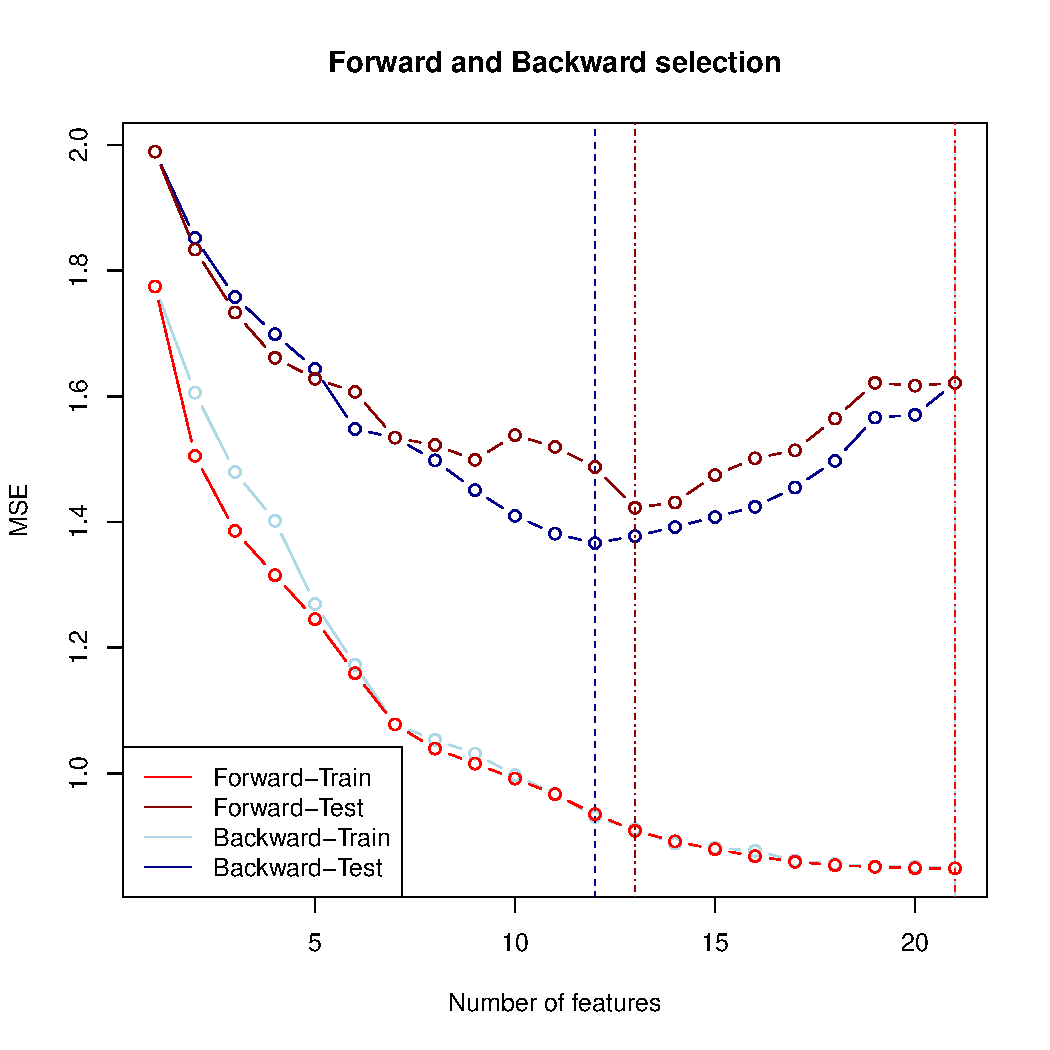
\includegraphics[width=\maxwidth]{figure/unnamed-chunk-5-1} 

\end{knitrout}
The train error is decreasing as the number of features grows because we allow more flexibility in the model. As for the test set, there is a minimum corresponding to the optimal trade off between how flexibile the model is and how many noise is added to it with useless features. We talk about overfitting when the model is too flexible.


\end{document}









